\documentclass[14pt,aspectratio=169,hyperref={pdftex,unicode},xcolor=dvipsnames]{beamer}
\usepackage[english,russian]{babel}
\usepackage[utf8x]{inputenc}
\usepackage[T2A]{fontenc}
\usepackage{cmap}
\usepackage{paratype}
\usepackage{hyperref}
\usepackage{minted} % для примеров кода (требует параметра -shell-escape)
\usepackage[hashEnumerators,smartEllipses]{markdown}

\usetheme{metropolis}
\usefonttheme[]{professionalfonts}  % запрещаем beamer'у перезаписывать мат. шрифты
\metroset{numbering=fraction}
\metroset{subsectionpage=progressbar}

\setbeamercolor{frametitle}{fg=black}
\setbeamertemplate{frametitle}
{
 \vspace{3mm}\insertframetitle\par
}
\setbeamertemplate{title separator}{}
\setbeamertemplate{footnote separator}{}


\usebackgroundtemplate{
\includegraphics[width=\paperwidth,height=\paperheight]{./common/background_white.jpg}}

\logo{\vspace{-1.2cm}
\includegraphics[width=6mm]{./common/short-v.pdf}\hspace*{1.08\textwidth}}

\institute
{
  \begin{columns}
    \begin{column}{1.5cm}
    
\includegraphics[height=15mm,keepaspectratio]{./common/math-cs.pdf}
    \end{column}
    \begin{column}{4cm}
          Факультет математики и компьютерных наук СПбГУ
    \end{column}
  \end{columns}
}


\begin{document}

\begin{frame}[plain]
  \begin{center}
    \textbf{Никита Митцев}

    {\Large\textbf{Исследование методов оценки производительности Projector}}

    

    {\small Руководитель проекта: Евгений Лазурин}

    24.05.2022
  \end{center}


  \begin{columns}
    \begin{column}{1cm}
    
\includegraphics[height=15mm,keepaspectratio]{./common/math-cs.pdf}
    \end{column}
    \begin{column}{10cm}
      \small
          Факультет математики и~компьютерных наук СПбГУ\\
          Программа <<Современное программирование>>, 2 курс
    \end{column}
  \end{columns}
\end{frame}



\begin{frame}
\frametitle{Что такое Projector}

\begin{itemize}
\item Современная JetBrains IDE потребляет много ресурсов
\item У больших компаний могут быть странные и строгие политики обращения с кодовой базой
\item Команда хотела сделать удобный удаленный доступ к среде разработке. В общем случае - к произвольному приложению на Swing.
\end{itemize}

\end{frame}

\begin{frame}
\frametitle{Постановка задачи}
\begin{enumerate}
  \item Команда не знает, как меняется производительность от версии к версии. Никаких измерений и тестов на начало работы не было.
  \item Летом планируется разработка полноценной системы оценки производительности.
\end{enumerate}
Ожидалось подготовить исследование в свободной форме: какие метрики хочется подсчитывать и что для этого нужно реализовать
\end{frame}

\begin{frame}{Часть 1: исследую поток данных}
  \begin{center}
    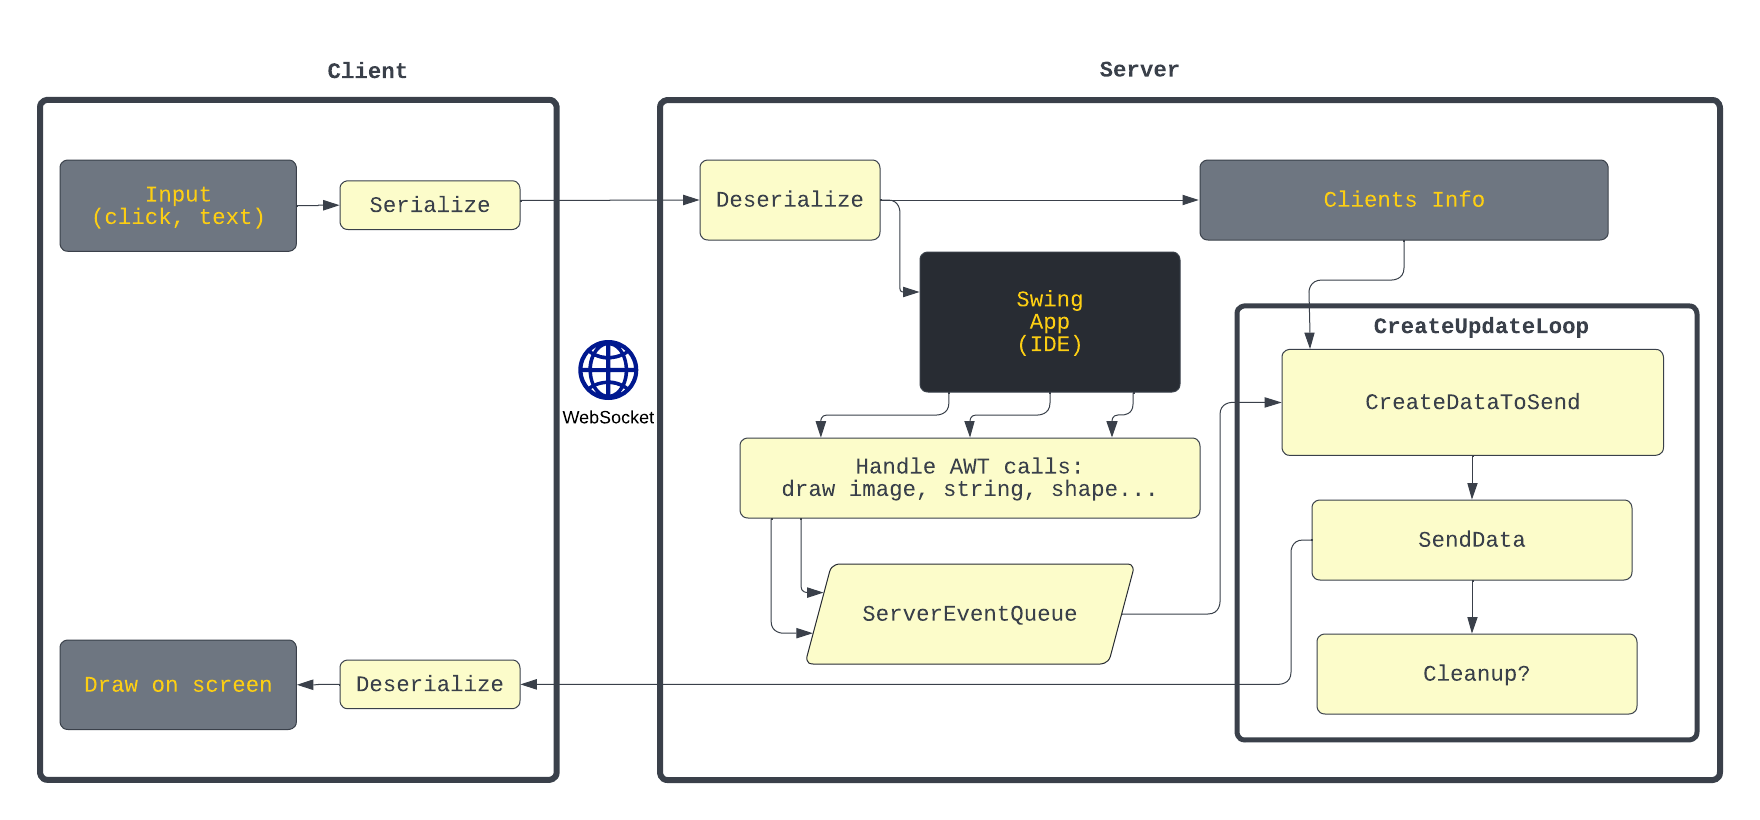
\includegraphics[width=14cm]{images/ProjectorFlowchartBetter.png}
  \end{center}
\end{frame}



\begin{frame}
  \frametitle{Автоматизация. Главные преграды}
  \begin{itemize}
    \item Подменить неконтролируемую JetBrains IDE на своё Swing приложение
    \item Запускать сервер с автоматическим подключением управляемого клиента
  \end{itemize}
\end{frame}


\begin{frame}
\frametitle{Генерация отчётов - графики}
\begin{center}
  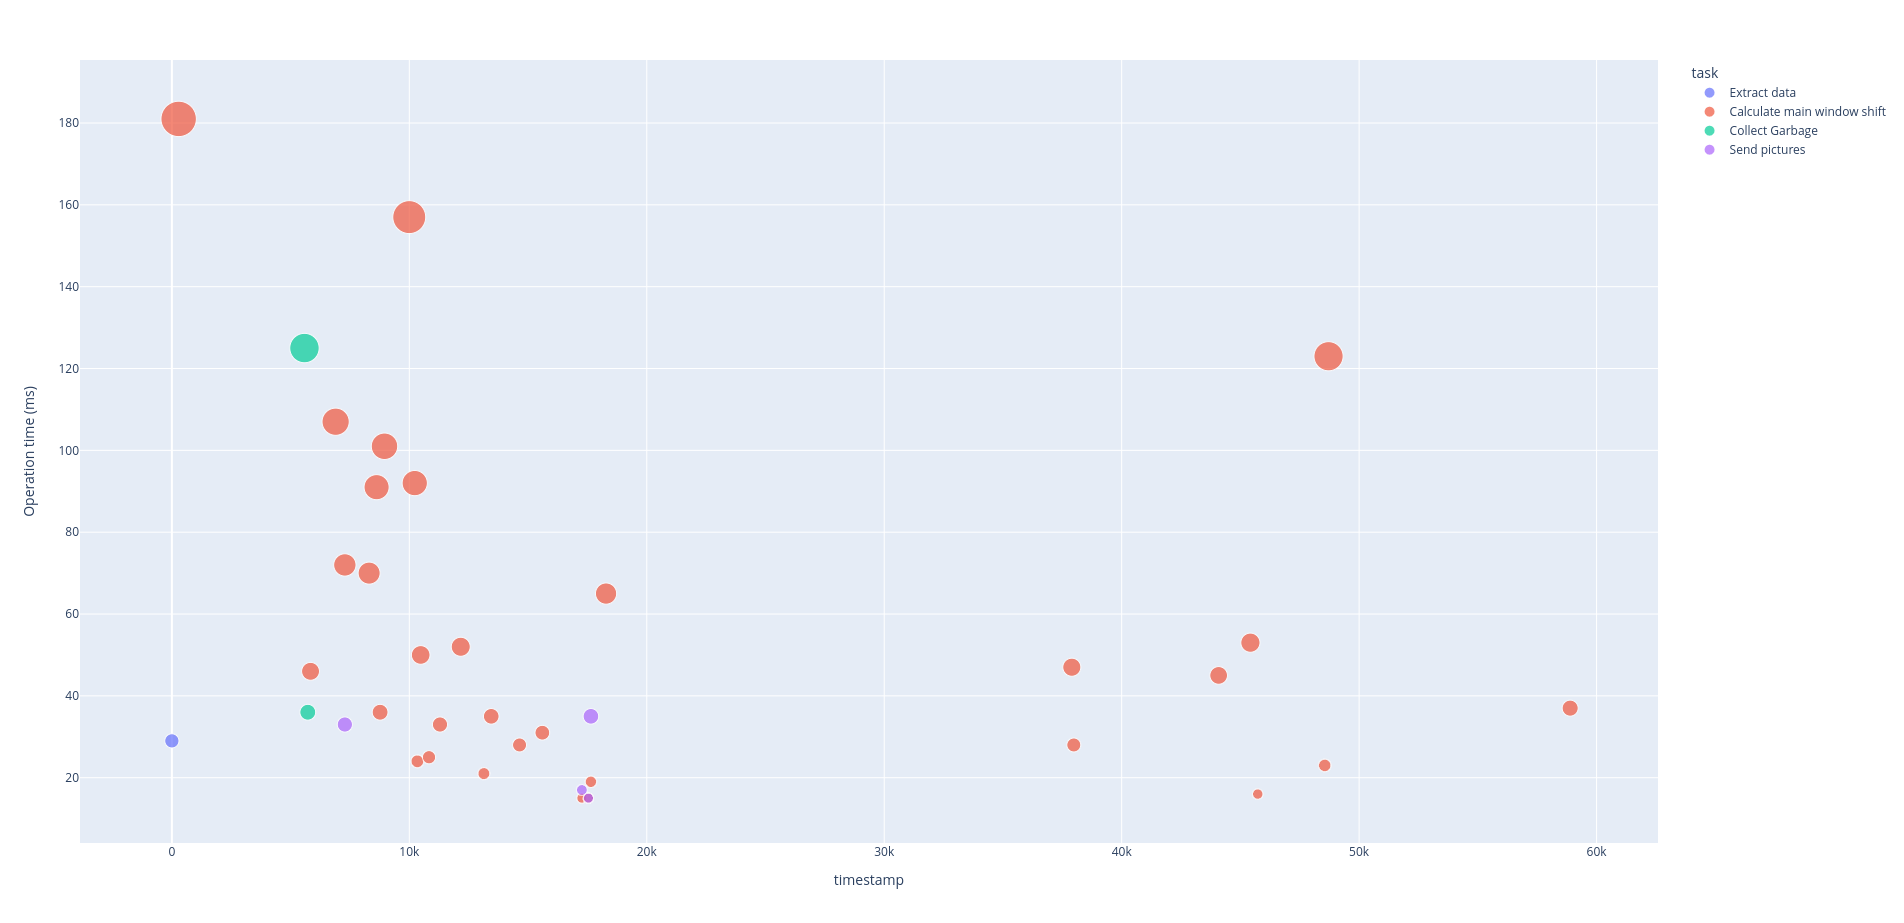
\includegraphics[width=14cm]{images/createUpdateThreshold.png}
\end{center}
\end{frame}

\begin{frame}
  \frametitle{Генерация отчётов: метрики}
  \scalebox{0.6}{
     
		\begin{tabular}{c|c|c|c|c}
			Name & Params & Measurement Unit & Value & Standard deviation \\
			\hline
			Average & minTime=0, minObj=0 & ms & 1 & 0 \\
			Peak rate & minTime=0, minObj=0 & millis / second & 110.3 & 2.4 \\
			Peak rate & minTime=3, minObj=0 & millis / second & 87 & 1.6 \\
			Peak rate & minTime=5, minObj=0 & millis / second & 80.7 & 2.5 \\
			Peak rate & minTime=10, minObj=0 & millis / second & 67 & 3.3 \\
			Peak rate & minTime=20, minObj=0 & millis / second & 54.3 & 4.2 \\
			Peak rate & minTime=3, minObj=2 & millis / second & 28.7 & 2.5 \\
			Peak rate & minTime=5, minObj=2 & millis / second & 27.3 & 2.9 \\
			Peak rate & minTime=5, minObj=3 & millis / second & 14 & 2.4 \\
			Power punishing rate & minTime=3, minObj=0 & (ms)^{1.2} / \text{second} & 177.7 & 5.3 \\
			Power punishing rate & minTime=5, minObj=0 & (ms)^{1.2} / \text{second} & 169 & 6.2 \\
			Power punishing rate & minTime=5, minObj=0 & (ms)^{1.5} / \text{second} & 559.3 & 22.9 \\
			Power punishing rate & minTime=5, minObj=0 & (ms)^{2.0} / \text{second} & 5047.7 & 190.9 \\
		\end{tabular}

  }
\end{frame}

\begin{frame}
\frametitle{Основные трудности}
\begin{itemize}
  \item Старые версии не поддерживаются и часто не собираются для сравнения
  \item Тяжело оценивать метрики, не имея возможности запускать приложение на контролируемом сценарии
  \item На любую метрику можно придумать такую ситуацию или оптимизацию, когда она не покажет изменений. Надо покрыть больше случаев, обойдясь малым количеством.
\end{itemize}

\end{frame}

\begin{frame}
  \frametitle{Результаты}
  \begin{itemize}
    \item Документ на англйском языке, где приведён анализ текущего состояния проекта и предложены решения по измерению различных показателей. Позже будет размещен в основном репозитории.
    \item Написан код для генерации графиков и отчётов по результатам запуска.
  \end{itemize}
  Всё это будет использовано далее как основа для создания полноценной системы профилирования проекта.
  
\end{frame}

\begin{frame}
  \frametitle{Ссылки}
  Автор: Никита Митцев, muldrik@yandex.ru\\
{\small
  \textit{Основной репозиторий проекта:} \href{https://github.com/JetBrains/projector-server}{https://github.com/JetBrains/projector-server}\\
  \textit{Репозиторий с кодом для сбора статистики:} \href{https://github.com/muldrik/projector-server}{https://github.com/muldrik/projector-server}\\
  \textit{Репозиторий с кодом для генерации отчётов и графиков:} \href{https://github.com/muldrik/projector-report-generator}{https://github.com/muldrik/projector-report-generator}
}
\end{frame}


\end{document}
